\documentclass[12pt,a4paper]{book}
\usepackage[utf8]{inputenc}
\usepackage[magyar]{babel}
\usepackage[T1]{fontenc}
\usepackage{amsmath}
\usepackage{amsfonts}
\usepackage{amssymb}

%\usepackage{URL}

\usepackage{multirow}
\usepackage{listings} %TODO configure for c#
\usepackage{cpp}
\usepackage{python}

\usepackage[left=2cm,right=2cm,top=2cm,bottom=2cm]{geometry}
\date{\vspace{-5ex}}

\usepackage{hyperref}

\usepackage{graphicx}

%TODO a petri háló írása legyen konzisztens a C# ahol lehet zenei # el legyen hivatkozva az az "official"
%TODO a tranzició rövid vagy hosszú i?


\title{BPEL üzleti folyamatmodellek korlátosság vizsgálata Petri-háló reprezentációval}

\begin{document}
%TODO re-include cover with images
%\begin{center}
\begin{tabular*}{\hsize}{@{}c@{\extracolsep{\fill}}c@{\extracolsep{\fill}}c@{}}
\multirow{2}[4]*{
\epsfig{file=images/ME_logo.eps,height=2truecm}}& \textcolor{blue}{\large\bfseries MISKOLCI EGYETEM}&\multirow{2}[4]*{
\epsfig{file=images/gepesz_logo.eps,height=1.6truecm}}\\
&\textcolor{blue}{\large\bfseries GÉPÉSZMÉRNÖKI ÉS INFORMATIKAI KAR}&\\
\end{tabular*}
\end{center}

\vglue 2.5truecm %függleges helykihagyás

\pagestyle{empty}

%A szakdolgozat címe, akár több sorban is
{\LARGE
\begin{center}
\textcolor{blue}{\Large\bfseries TDK DOLGOZAT}
\end{center}}

\vspace*{2.5truecm}
\begin{center}
% (Tag Based Document Management)
\LARGE\bfseries BPEL üzleti folyamatmodellek korlátosság vizsgálata Petri-háló reprezentációval
\end{center}
\vglue 2cm

{\large
\begin{center}
\begin{tabular}{c}
{\bfseries Hornyák Bence}\\
Programtervező informatikus BSc
\end{tabular}
\end{center}
\vglue 3cm
\begin{center}
\textbf{Konzulens:}
\end{center}
\medskip
\begin{center}
\begin{tabular}{ccc}
\textbf{Dr. Kovács László} \\
tanszékvezető, egyetemi docens \\
Általános Informatikai Tanszék \\
\end{tabular}
\end{center}
\vfill
{\large

\begin{center}
\textbf{\textsc{Miskolc, 2019}}
\end{center}}

\newpage
\newpage
\tableofcontents

%TODO Add motivation, structure, results


\chapter{Bevezetés}
A BPEL (\textit{Business Process Execution Language}) nyelv létrejötte elsődlegesen a Web szolgáltatások területéhez kapcsolódik, de a nyelv mint általános munkafolyamat (\textit{workflow}) leíró nyelv, más alkalmazási témakörhöz is köthető. A BPEL szerepét fontosságát, jól mutatja az a tény is, hogy igen gazdag irodalom található az egyes alkalmazási területekről és speciális szabvány kiegészítésekről.
%TODO Ide kellenének a hivatkozások néhány irodalomról!

A  BPEL aktualitását jelzi, hogy a megvalósító motorok köre is folyamatosan bővül. Ugyan már lassan 15 év eltelt a szabvány bevezetése óta, a meglévő nagyobb rendszerek (Oracle BPEL Process Manager, IBM WebSphere Process Server, Microsoft BizTalk Server, SAP SAP Exchange Infrastructure) alternatívájaként  most is jelennek meg új végrehajtó motor implementációk. A Wikipédia forrása szerint \cite{wikiBpelList} a közelmúltban az alábbi szabad szotver implementációk születtek (\ref{tab:bpel_softwares}. táblázat).

\begin{table}[h!]
\centering
\caption{A BPEL nyelv szabad szoftveres implementációi.}
\label{tab:bpel_softwares}
\begin{tabular}{|c|c|c|c|}
\hline
\textbf{Termék neve} & \textbf{Fejlesztő} & \textbf{Megjelenés éve} & \textbf{Licensz}\\
\hline
JBPM & JBoss & 2016 & Apache\\
Apache ODE & ASF & 2016 & Apache\\
Activiti & Alfresco & 2014 & Apache\\
\hline
\end{tabular}
\end{table}

Annak ellenére, hogy napjainkra már több BPEL motor elérhető és használatos, a BPEL szerkesztők és különösen a BPEL validációs rendszerek köre igen szegényes. Ezen tapasztalatokból kiindulva a dolgozat célja egy olyan BPEL validációs rendszer elkészítése, amely a BPEL rendszerek egyik fontos tulajdonságát, a terhelés korlátosságát (\textit{bounded model})
%TODO Be kellene hivatkozni, hogy hol hívják ezt bounded modelnek!
vizsgálja. A korlátosság azt jelzi, hogy minden csomópontban van egy felső korlát a végrehajtható feladatok számára, intenzitására vonatkozóan. Ha a rendszer nem teljesíti ezt a kritériumot, akkor túlcsordul valamely megmunkáló/tároló helyen. Az elemzés során a korlátosság ténye mellett, a korlát értékei is fontos vizsgálandó jellemzők. 

A meglévő tervezői rendszerekben legtöbbször szimulációval történik a főbb paraméterek, a korlátosság vizsgálata. Ezen megközelítésnek rendszerint két problémája van: az vizsgálat teljessége (azaz valóban minden lehetséges esetet áttekintettük-e) illetve a végrehajtási idő (a szimulációk futtatása hosszabb időt is igénybe vehet).

A dolgozatban a BPEL folyamatok Petri-háló alapú vizsgálatát végzem el. A Petri-háló alapú reprezentáció egy elfogadott és többek által alkalmazott megközelítés. A kidolgozott rendszer inputként egy  BPEL modell leírását várja és kimenetként az elemzés eredményét illetve a folyamatok nyomkövetését adja vissza.
 %ch1-Introduction
%TODO Add bpel control elements, 10 example from core std /w pics, annot, and bpel desgn pictograms. Non core elements only w/ annotation

\chapter{A BPEL és folyamatainak bemutatása} 

A BPEL (Buisness Process Execution Language)üzleti folyamatok végrehajtó nyelve \cite{saraswathi2013oracle}.
Az OASIS által kezelt XML alapú szabványt használ. 
A dokumentum felépítésében egy XML dokumentum, mely a WS-BPEL szabvány szerint validált. A BPEL programok szerkezetét célszerű egy mintával áttekinteni, a jobb megértéshez. %TODO link: http://docs.oasis-open.org/wsbpel/2.0/OS/wsbpel-v2.0-OS.html chapter 5 section 1
Vegyük a következő példát.  \textsl{Adott egy online rendelést felvevő cég. A cég egy automata segítségével generál számlákat A számla az ár kiszámítása, a futár kiválasztása, és a szükséges termelés ütemezése után kerül kiállításra.} A lépéseket az alábbi ábra mutatja be: %TODO insert fig1.png 
Az ábrán a téglalapok egy rész processzt jelentenek. Az egy blokkban különállóak pedig konkurens proceszeket. A szaggatott vonal szekvenciát jelöl, míg a teli/sima pedig vezérlő linkek, a konkurens processzek szinkronizációját, várakoztatását lehet velük megoldani. Az ábra nem képez átíratot, csak mint egy standard érthető vizualizáció segíti a megértést. 

A program következő része egy WSDL szabvány ami a portot adja meg a processz számára. %TODO link to appendix
\newpage


 
 A kódban szereplő \texttt{<partnerLinks>} tartalmaz mindent (így közvetetten mindenkit) amik kapcsolatba kerül a processzel. Az elnevezés tükrözi a résztvevő partit, valamint a résztvevő feladatát, szándékát. A \texttt{<variables>} a változókat tartalmazza, míg a \texttt{<faultHandlers>} a hibakezelőket. A hibakezelés egy try-catch-finally "hibakezelőblokk" helyett az XML mentalitását tükröző módon kerül lekezelésre, a handlerek által. A kód többi része a processz standard definíciójához tartozik. A példák alapján elmondható, hogy a program a következő struktúra szerint épül fel.
\begin{itemize}
\item \textbf{Definíció: } a processz neve, névtere és különféle sémahívások, majd bővítmények, importok
\item \textbf{PartnerLinkek: } A megfelelő partnerek hozzáadása attribútumokkal. 
\item \textbf{Változók}
\item \textbf{Hibakezelők}
\item\textbf{Eseménykezelők}
\end{itemize}
%ch2-BPEL-introduction, 
\chapter{Petri-hálók és alkalmazásaik}
\section{Az alap Petri-hálók}
A Petri-háló egy matematikai leírómodell elosztott rendszerek bemutatására.
A modellt Carl Adam Petri készítette.
A modell nagyon hasonlít a programozók körében elterjedt folyamat ábrára.
A háló irányított élekből, helyekből és átmenetekből (\textsl{mint elemek}) áll.
Az élek csak két különböző típusú elem között állhatnak.
A helyeken pontok, ún. tokenek állhatnak.
A tokenek csak diszkrét számban fordulhatnak elő egy helyen, és a token átvitele atomi folyamat, azaz nem félbeszakítható.
A tokenek elláthatóak attribútummal is ilyen esetben a tokeneket "kiszínezzük" és színezett petri hálóról beszélünk. (ld. 2.2.) %TODO (LINK!)

%TODO cite: https://www.abhishekhalder.org/PetriNetReport.pdf__vq9vUXcOjS%2BawepkKcMLeAA64c19da3fb4d67754c3fe7eba8ce1187
Az alap Petri háló egy biparit, irányított és súlyozott multigráf $PN(P,T,A,W,S)$, ahol 
\begin{itemize}
\item $P=\{ p_1,p_2,\ldots ,p_N \}:$ a helyek véges halmaza ,
\item $T=\{ t_1,t_2,\ldots ,t_M\}:$ egy véges tranzició halmaz,
\item $P\cap T = \emptyset$
\item $A \subseteq P\times T \cup T\times P:$ az élek halmaza,
\item $W: F\Rightarrow N^+:$ az élsúlyok halmaza
\item $S: P\Rightarrow N^+:$ a kezdőállapot.
\end{itemize}

\section{Színezett Petri-hálók}

Az elemi színezett háló felírható, mint egy oly struktúra, ami: $CPN(P,T,A,\Sigma ,V,C,G,E,S)$, ahol 
\begin{itemize}
\item $P=\{ p_1,p_2,\ldots ,p_N \}:$ a helyek véges halmaza ,
\item $T=\{ t_1,t_2,\ldots ,t_M\}:$ egy véges tranzició halmaz,
\item $A \subseteq P\times T \cup T\times P:$ az élek halmaza,
\item $\Sigma:$ a színek halmazainak halmaza, 
\item $V:$ a változók halmaza, ahol $\forall v\in V:$ változóhoz egy $Type[v] \in \Sigma $ típus rendelhető,
\item $C: P\rightarrow \Sigma :$ a helyekhez színeket rendelő függvény,
\item $G: T\rightarrow EXPR_V:$ az egyes tranzíciókhoz kapcsolódó validációs, ellenőrzési kifejezés (logikai értékű)
\item $E: A\rightarrow EXPR_V:$ z  egyes élekhez kapcsolódó kifejezés, amely a kapcsolódó hely színhalmazához tartozó értéket vehet fel
\item $S: P\Rightarrow N^+:$ a kezdőállapot.
\end{itemize}

Adott $CPN(P,T,A,\Sigma ,V,C,G,E,S)$ színezett hálóhoz az alábbi kezelő funkciók köthetőek: 
\begin{itemize}
\item $M(p):$ a jelölő (marker) függvény, melynek értéke a $p$ helyhez kapcsolódó tokenek halmaza. Színezett Petri háló esetén az $M(p)$ elemek színeinek illeszkedni kell a $C(p)$ színhalma
\item $M_0(p):$  helyek induló tokenkészlete
\item $Var(t):$ a tranzíciók viselkedését leíró változók halmaza
\item $b(v):$ a adott v változó értékét megadó kifejezés, ahol $b(v) \in Type[v]$
\end{itemize}

Egy adott $t$ tranzíció esetén a $Var(t)$ kifejezés a tranzícióhoz rendelt változók együttese, ahol a változók a $G(t)$ vagy $E$(a: t-hez kötődő él) kifejezésekben szerepelnek.
\begin{equation*}
Var(t)=\begin{cases}
\{n,d\} &\text{if } t=SendPacket\\
\{n,d,success\} &\text{if } t= TransmitPacket\\
\{n,d,k,data\} &\text{if } t=ReceivePacket\\
\{n,success\} &\text{if } t=TrancmitAck\\
\{n,k\} &\text{if }t=ReceiveAck
\end{cases}
\end{equation*}

A hálóban egy tranzíció akkor engedélyezett (ready), ha minden bemenő helyeknél a kívánt tokenszám megtalálható.   Jelölt hálók esetében:
$$M'(p)=M(p)-I(p,t)+O(p,t): \forall p\in P,$$ ahol 
\begin{itemize}
\item $I:F\Rightarrow N^+:$  bejövő áram intenzitás
\item $O:F\Rightarrow N^+:$ kimenő áram intenzitás

\end{itemize}
A hierarchikus CPN rendszerben az átláthatóság növelése érdekében összefogó modulokat is lehet alkalmazni. Egy modul más elemi egységek együttese, konténere. %TODO Insert "rendszerséma 3 modullal.png" & 2A receiver belső szerkezete.png"

A moduloknál fontos szerepet kapnak az átadó helyek, melyeken keresztül a tokenek bejöhetnek a modulba illetve kiléphetnek a modulból. Az ilyen port jellegű helyek lehetnek bemeneti portok (IN) illetve kimeneti portok (OUT).  

A CPN rendszerek egyik hasznos tulajdonsága, hogy lehetőséget adnak a felépített modell formális ellenőrzésére, validálására és értékelésére. A formális ellenőrzés egyik leggyakoribb eszköze az állapottér (state space)  modell, ahol az állapottér egy olyan irányított gráf, melyben a csomópontok a háló egy lehetséges  M(CPN) jelölési állapota. Azaz a háló struktúrája rögzített, de az egyes elemeknél a tokenek és változók halmaza, azok állapota változhat. A véges állapottér modellt rendszerint szimulációkal állítják elő. 

Az állapottér modellből kiindulva további elemzésekre ad lehetőséget a komponens gráf modell (SCC graph:  strongly-connected-component graph) formalizmus. Az  SCC gráfból a rendszer általános viselkedési szabályaira lehet következtetni. Az SCC gráf olyan gráf, melynek csomópontjai  az állapottér azon diszjunkt részhalmazai, ahol egy részhalmaz bármely két elemére igaz, hogy az egyik elem  elérhető a másikból. 

Az elemzések során az alábbi főbb tulajdonságok elemzésére szoktak kitérni:
\begin{itemize}
\item Reachability Properties
\item Boundedness Properties
\item Home Properties 
\item Liveness Properties
\item Fairness Properties
\end{itemize}
%TODO insert mintaállapottér 1-2-3.png here

%ch3 Petri net definition+intorduction
\chapter{Az üzleti folyamatok elemeinek leképzése}

%TODO Ide kellene felsorolni, és részletesen leírni, hogy a BPEL egyes elemeinek milyen Petri-háló feleltethető meg.

%TODO Megnézni, hogy az egyes elemek esetében milyen alternatívák lennének a leképzésre!
\section{A leképzés menete}
A BPEL nyelv az egymással együttműködő modulok működését szimulálja. A BPEL  modellben a folyamat lépéseit tevékenységnek \textsl{activity} nevezzük. A tevékenységek lehetnek elemiek és összetettek. Tipikus elemi tevékenységek:
\begin{itemize}
\item más funkció meghívása,
\item üzenet küldés/fogadás,
\item változók módosítása,
\item várakozás, szinkronizálás.
\end{itemize}
Az elemi tevékenységekből összetett folyamatok építhetőek fel szekvencia, párhuzamosítás és ciklus elemek segítségével.

A BPEL szabvány tevékenység készletének bemutatásánál csak a legfontosabb elemekre térünk most ki. A szabvány részletei a
http://docs.oasis-open.org/wsbpel/2.0/OS/wsbpel-v2.0-OS.html weboldalról érhetőek el. 

A BPEL definíció egyértelműsíti a folyamat kezdetét és inicializálja is a megfelelő paraméterekkel. A Petri háló erre nem tér ki, ezért bevezetünk egy opcionális \textit{START} tranazíciót. Ennek feladata, a megfelelő tokenek legenerálása a folyamat indításához. A folyamat zárása szintén egyértelmű a BPEL szabványban. Petri háló kapcsán beszélhetünk a háló leállásáról, ha már semmilyen hely és tranzíció nem produkál új tokent, nem várakozik és nem nyel el tokent. A köztes elemek leképzése általánosan nem bonyolult, de megvizsgálhatók alternatív leképzési módok. 

Az alkalmazás jelölésrendszere: A rendszer a helyeket P-vel, míg a tranzíciókat T-vel indexeli. A helyek után listázza az adott helyen levő tokeneket. A jelenleg lépésben levő tranzíciók pedig színes kitöltést kapnak.

\section{\texttt{<receive>}}

Egy megfelelő üzenet után engedi a folyamatot továbbhaladni, így várakoztatáshoz használható. A \texttt{<receive>} típusú XML elemekhez tartozó sémaleírás:\\
\begin{verbatim}
<receive partnerLink="NCName"
   portType="QName"?
   operation="NCName"
   variable="BPELVariableName"?
   messageExchange="NCName"?>
   <fromParts>?
      <fromPart part="NCName" toVariable="BPELVariableNm"/>+
   </fromParts>
</receive>
\end{verbatim}
A hálóban ezt egy tranzicióval könnyedén megoldhatjuk, hiszen csak egy specifikus üzenet token kell a továbblépéshez, és a többit addig az előző helyen parkoltatja. 

\section{\texttt{<reply>}}
Üzenetküldő elem, ami \texttt{<receive>; <onMessage>;<onEvent>} események után léphet akcióba. 
\begin{verbatim}
<reply partnerLink="NCName"
   portType="QName"?
   operation="NCName"
   variable="BPELVariableName"?
   messageExchange="NCName"?>
   <toParts>?
      <toPart part="NCName" fromVariable="BPELVariableNm"/>+
   </toParts>
</reply>
\end{verbatim}
A lekezelése az előző példával analóg módon, annyi különbséggel, hogy a tokenek nem parkolnak, hanem tovább mennek és a tranzíció csak akkor generál új tokent ha üzenetet kap egy ágról.

\section{\texttt{<invoke>}}
Egy BPEL vagy épp egy webszolgáltatás meghívására szolgál és definiálja a szolgáltatás feladatát is. 
\begin{verbatim}
<invoke partnerLink="NCName"
   portType="QName"?
   operation="NCName"
   inputVariable="BPELVariableName"?
   outputVariable="BPELVariableName"?>
   <catch faultName="QName"? … >*
  	activity
   </catch>
   <toParts>?
      <toPart part="NCName" fromVariable="BPELVariableNm"/>+
   </toParts>
   <fromParts>?
      <fromPart part="NCName" toVariable="BPELVariableNm"/>+
   </fromParts>
</invoke>
\end{verbatim}
A grafikus megjelenítése \aref{fig:invoke}. ábrán látható.

\begin{figure}[h!]
\centering
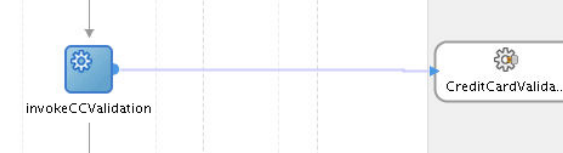
\includegraphics[scale=0.6]{images/invoke.png}
\caption{Az \texttt{invoke} grafikus jelölése az Oracle BPEL designer-ben}
\label{fig:invoke}
\end{figure}

Használatát a programrészek újrafelhasználhatósága indokolja, valamint az átláthatósági alapelvek. Például, az ábrán látható CCvalidation használható ATM-es pénz felvét, egyenleglekérdezés, vagy egyéb ATM nél végezhető művelet során. 

\begin{figure}[h!]
\centering
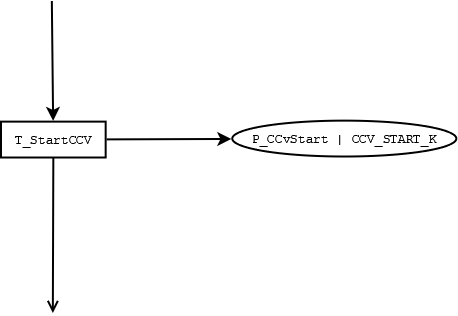
\includegraphics[scale=0.4]{images/invokenet.png}
\caption{Az \texttt{<invoke>} leképzése petri hálóra}
\label{fig:invokenet}
\end{figure}
Leképzés során ügyelni kell arra, hogy az \texttt{invoke} paramétereinek megfelelő tokenek keletkezzenek és legyenek átadva a részháló start elemének.

\section{\texttt{<assign>}}

Egy változó értékadására szolgáló esemény. Ellentétben egy imperatív értékadással egy \texttt{<assign>} blokkban bármennyi értékadás, másolás történhet, amíg azt a kliens kezelni tudja, így logikailag egy egységbe zárja a műveleteket.  
\begin{verbatim}
<assign validate="yes|no"? standard-attributes>
   (
   <copy keepSrcElementName="yes|no"? 
  	from-spec
  	to-spec
   </copy>
</assign>
\end{verbatim}
Az érték hozzárendelése nagyon egszerűen átírható egy tranzicióra ami a megfelelő tokenek színét módosítja. 
A grafikus megjelenítése \aref{fig:assign}. ábrán látható.
A színmódosítás egyszerűen a token nevének átírását jelenti. 
\begin{figure}[h!]
\centering
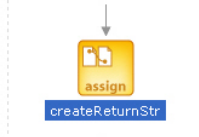
\includegraphics[scale=1]{images/assign.png}
\caption{Az \texttt{assign} grafikus jelölése az Oracle BPEL designer-ben}
\label{fig:assign}
\end{figure}

\begin{figure}[h!]
\centering
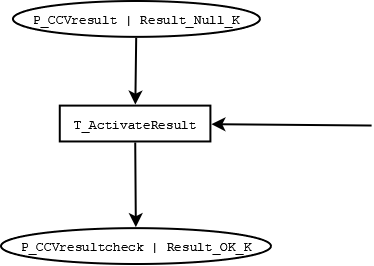
\includegraphics[scale=0.4]{images/assignnet.png}
\caption{Az \texttt{assign} leképzése petri hálóra}
\label{fig:assignnet}
\end{figure}
Az ábrán egy változós értékadásra látható példa. Hasonló módon kezelendő a  blokkosított értékadás, a különbség, hogy a több token jöhet és távozhat több forrásba is.

\section{\texttt{<validate>}}
Egy sémára validálja az XML (BPEL) állományt. 
\begin{verbatim}
<validate variables="BPELVariableNames" standard-attributes>
   standard-elements
</validate>
\end{verbatim}
Mivel a Petri háló nem tartalmaz validációs elemeket, ezért a \texttt{<validate>} nem képződik le. 

\section{\texttt{<throw>}}
Egy rész processzen belül fault generálására szolgál. 
\begin{verbatim}
<throw faultName="QName"
   faultVariable="BPELVariableName"?
   standard-attributes>
   standard-elements
</throw>
\end{verbatim}
Nagyon egyszerűen egy \textit{fault} tokent generáló tranzició komponens. Explicit hálórésze nincs, hanem a megfelelő inputtokenek megléte vagy hiánya generálja egy tranzició során. 

\section{\texttt{<wait>}}
Időre vonatkoztatva várakoztat. Például 5000 tick vagy 14:00:23 (hh:mm:ss)
\begin{verbatim} 
<wait standard-attributes>
   standard-elements
   (
   <for expressionLanguage="anyURI"?>duration-expr</for>
   |
   <until expressionLanguage="anyURI"?>deadline-expr</until>
   )
</wait>
\end{verbatim}
Megadható egy részhálóval ami valójában egy oszcillátor és a megfelelő iteráció után folytat tokent küld. Továbbá létezik úgynevezett időérzékeny háló, ahol az elemek tokenátadási sebessége ismert, vagy állítható. Ezzel időzítőt lehet létrehozni. Esetenként hardware-es óra is használható

\section{\texttt{<empty>}}
No-op (\textit{no operations}) esemény szinkronizációra szolgál.
\begin{verbatim}
<empty standard-attributes>
   standard-elements
</empty>
\end{verbatim}
Beiktatható egy semleges tranzició és hely.

\section{\texttt{<sequence>}}
Sorozatot ad meg.
\begin{verbatim}
<sequence standard-attributes>
   standard-elements
   activity+
</sequence>
\end{verbatim}
Egyszerűen csak tranziciók és helyek összefűzése. 

\section{\texttt{<if>}}

\texttt{<if>} Standard kétirányú elágazás. Logikai XPATH kifejezést vár. 
\begin{verbatim}
<if standard-attributes>
   standard-elements
   <condition >bool-expr</condition>
   activity
   <elseif>*
      <condition>bool-expr</condition>
  	activity
   </elseif>
   <else>?
  	activity
   </else>
</if>
\end{verbatim}
Egy tranzició, mely tokenek függvényében más felé küldi tovább, vagy generál tokeneket. Ez lehet egy helyen összegyúlt tokenek mennyisége, vagy egy adott helyen egy specifikus színű token megléte, vagy nemléte. Analóg módon egy \textit{Switch-Case} elágazás is definiálható vele.
A PBEL-es grafikus megjelenítése \aref{fig:if}. ábrán látható.

\begin{figure}[h!]
\centering
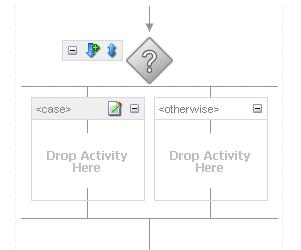
\includegraphics[scale=1]{images/if.png}
\caption{Az \texttt{if} grafikus jelölése az Oracle BPEL designer-ben}
\label{fig:if}
\end{figure}


\begin{figure}[h!]
\centering
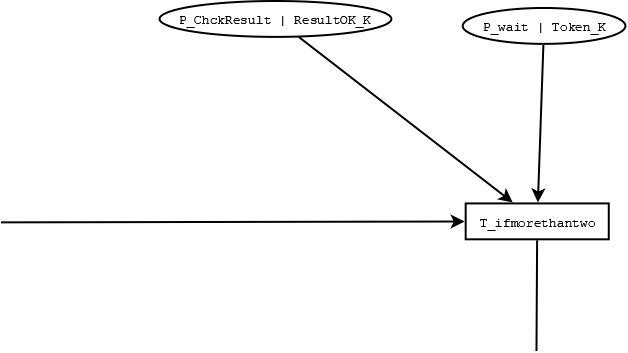
\includegraphics[scale=0.4]{images/ifnet.png}
\caption{Az \texttt{if} Egy hálóképzése}
\label{fig:ifnet}
\end{figure}

\section{\texttt{<while>}}
Elöltesztelős ciklus. Addig iterál, amíg az ciklus feltétel igaznak értékelődik ki. 
\begin{verbatim}
<while standard-attributes>
   <condition>bool-expr</condition>
   activity
</while>
\end{verbatim}
Egy tranzició, mely token függvényében a folyamat egy korábbi pontjára csatol vissza, vagy éppen egy későbbire, a feltétel hamis logikai állapota esetén. A feltétel persze egy színes token jelenléte, vagy tokenek száma is lehet. 

\section{\texttt{<repeatUntil>}}
Egy hátultesztelős ciklusnak feleltethető meg, amely akkor enged tovább, ha a feltétel igaz. 
\begin{verbatim}
<repeatUntil standard-attributes>
   standard-elements
   activity
   <condition expressionLanguage="anyURI"?>bool-expr</condition>
</repeatUntil>
\end{verbatim}
A \texttt{<while>}-al analóg módon megadható a Petri-hálós leképzése.

\section{\texttt{<forEach>}}
Végig iterál a gyerekelemeken. Megadható párhuzamos feldolgozás is. Egy \textit{Complete condition} segítségével megadható egy break utasítás ami kilép a ciklusból. 
\begin{verbatim}
<forEach counterName="BPELVariableName" parallel="yes|no">
   <startCounterValue expressionLanguage="anyURI"?>
  	unsigned-integer-expression
   </startCounterValue>
   <finalCounterValue expressionLanguage="anyURI"?>
  	unsigned-integer-expression
   </finalCounterValue>
</forEach>
\end{verbatim}
Egyszerű loop utasítás, azonban párhuzamosítás esetén a részhálóból megfelelő példányszámot generáltatunk. 

\section{\texttt{<pick>}}
Üzenetek várására vagy időtúllépés eseményre figyel. Ezek bármelyike a szubprocessz végrehajtásához vezet. 
\begin{verbatim}
<pick createInstance="yes|no"? standard-attributes>
   standard-elements
   <onMessage partnerLink="NCName"
      portType="QName"?
      operation="NCName"
      variable="BPELVariableName"?
      messageExchange="NCName"?>+
      <correlations>?
         <correlation set="NCName" initiate="yes|join|no"? />+
      </correlations>
      <fromParts>?
         <fromPart part="NCName" toVariable="BPELVariableName" />+
      </fromParts>
      activity
   </onMessage>
   <onAlarm>*
      (
      <for expressionLanguage="anyURI"?>duration-expr</for>
      |
      <until expressionLanguage="anyURI"?>deadline-expr</until>
      )
      activity
   </onAlarm>
</pick>
\end{verbatim}
A grafikus megjelenítése \aref{fig:pick}. ábrán látható.

\begin{figure}[h!]
\centering
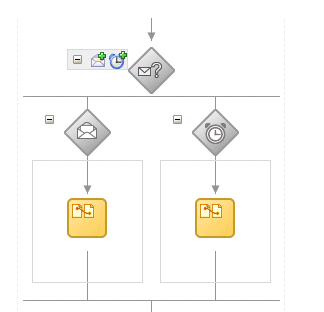
\includegraphics[scale=1]{images/pick.png}
\caption{A \texttt{pick} grafikus jelölése az Oracle BPEL designer-ben}
\label{fig:pick}
\end{figure}

Összetartó hálóval és egy tranzícióval képezhető le.


\section{\texttt{<flow>}}

Konkurens elemek deklarálására szolgál. Linkek segítségével megadható függőségi viszony a gyerekek között. 
\begin{verbatim}
<flow standard-attributes>
   standard-elements
   <links>?
      <link name="NCName" />+
   </links>
   activity+
</flow>
\end{verbatim} 
A grafikus megjelenítése \aref{fig:flow}. ábrán látható.

\begin{figure}[h!]
\centering
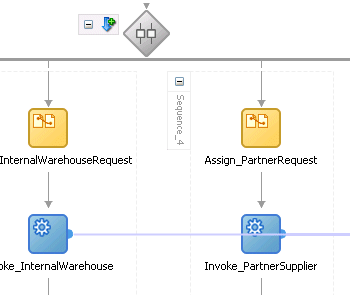
\includegraphics[scale=1]{images/flow.png}
\caption{A \texttt{flow} grafikus jelölése az Oracle BPEL designer-ben}
\label{fig:flow}
\end{figure}
Leképzése egyszerű, hisz a megfelelő gyerek elemek nem szekvenciálisan helyezkednek el, hanem párhuzamosan.
\section{\texttt{<scope>}}

A gyerek elemek hatókörét lehet vele szabályozni.
\begin{verbatim}
<scope isolated="yes|no"? exitOnStandardFault="yes|no"?
   standard-attributes>
   standard-elements
   <partnerLinks>?
      ... see above under <process> for syntax ...
   </partnerLinks>
   <messageExchanges>?
      ... see above under <process> for syntax ...
   </messageExchanges>
   <variables>?
      ... see above under <process> for syntax ...
   </variables>
   <correlationSets>?
      ... see above under <process> for syntax ...
   </correlationSets>
   <faultHandlers>?
      ... see above under <process> for syntax ...
   </faultHandlers>
   <compensationHandler>?
      ...
   </compensationHandler>
   <terminationHandler>?
      ...
   </terminationHandler>
   <eventHandlers>?
      ... see above under <process> for syntax ...
   </eventHandlers>
   activity
</scope>
\end{verbatim}
Nem generál új elemet, csak a láthatósági, azaz visszacsatolási elemeket adja meg. 


%ch4 BPEL to Petri net and annotations
\chapter{Szimulációs keretrendszer}

%TODO Be kell mutatni a C# nyelvű alkalmazást.

\section{Elvárások az alkalmazással szemben}

%TODO Itt kellene röviden áttekinteni az alkalmazással szemben támasztott követelményeket.
Az alkalmazás legfőbb feladata egy konverzió, BPEL és Petri-háló között. Ebből adódóan minden BPEL elemet le kell tudnia kezelni, illetve az azok közti összefüggéseket feltérképezni, és az összefüggés halmazból egy petri hálót előállítani. A hálót tudni kell megjeleníteni, valamint a hálón belüli mozgásokat rajzolni, és szükségesség esetén input file-t vagy felhasználói inputot kezelni. Ha a háló nem hozható létre, akkor azt tudatnia kell,és lehetőség szerint rövid indoklással alátámasztania. 

\section{Az alkalmazás felépítése}

%TODO Osztály és blokkdiagramok formájában be kellene mutatni, hogy milyen fő elemekből épül fel az alkalmazás.
Az alkalmazás logikailag a következő fő részekből áll:
\begin{itemize}
\item I/O module: Beolvassa az XML dokumentumot és felparseolja. Szükség esetén menti a kész hálót.
\item Conversion module: Átkonvertálja  a beolvasott dokumentumot.
\item Data Structure module: A saját típusú Petri elemeket kezeli, és adatszerkezeti implementációt tartalmaz. 
\item UI talker: A UI ra illeszti a megfelelő input mezőt, az abba felvitt értéket átadja a feldolgozó egységnek.
\item Graphics module: Az MSGL libraryre épül. Feladata a gráf rajzolása és megjelenítése animációval együtt. 
\item Computing module: A háló animációjához végzi a szükséges számításokat és időzítéseket. 
\end{itemize}

\section{C\# implementáció}

%TODO Meg kellene mutatni, hogy milyen API és újrahasznosítható elemek készültek el.

\section{Tesztelés, tapasztalatok}

%TODO Itt kifejezetten az alkalmazás szemszögéből (nem pedig üzleti folyamatokra vonatkozóan) kellene bemutatni az alkalmazást.
%ch5 The definiton and logic of the framework
\chapter{Az alkalmazás implementációja}
\section{C\# implementáció}
% Meg kellene mutatni, hogy milyen API és újrahasznosítható elemek készültek el.
Az alkalmazás implementációja során fontos volt a C\# alapelveinek betartása (OOP elvek és nyelv specifikus elvek együttvéve). Szerencsére nem kellett újra feltalálni semmit, hisz a .NET rendelkezik Gráf rajzolóval, megjelenítővel, (hozzá különféle szolgáltatásokkal) és különféle standard formátumú fileokra készített feldolgozó modulokkal. Ebből adódóan a lényeges munka az átalakító modulok és az adatstruktúrák megírása volt. 
\begin{cpp}
internal class Model
    {
        public class Net
        {
            public List<Place> Places { get; set; }
            public List<Transition> Transitions { get; set; }
            public List<Arc> Arcs { get; set; }

            public Net()
            {
                Places = new List<Place>();
                Transitions = new List<Transition>();
                Arcs = new List<Arc>();
            }
        }

        public class Node
        {
            public string Label { get; set; }
        }

        public class Place : Node
        {
            public List<Token> Tokens { get; set; }
        }

        public class Transition : Node
        {

        }
        public class Arc
        {
            public Node Input { get; private set; }
            public Node Output { get; private set; }
            public int Multiplicity { get; set; }
        }

        public class Token
        {
            public string Color { get; set; }
        }
    }
\end{cpp}
\textsl{A Színezett Petri-háló adatstruktúrája}

A step-by-step animáció úgy készül, hogy a megfelelő lépések legenerálódnak. A képek bekerülnek egy pipe-ba, ami a program beállításaiban megadott időzítő ütemére átadásra kerülnek megjelenítésre. 
A lépések addig számítódnak amíg a folyamat teljes egészében lefut, vagy egy olyan nodehoz nem ér ami felhasználói bevitelt vár. Ekkor a számítás szünetel és a UI megjelenítő előkészít egy input mezőt. Az input mező a felhasználói adatbevitel után (ha nem szükséges a következő lépéshez) eltűnik, az átláthatóság kedvéért. A mező tartalma átkerül feldolgozásra és általában token formájában kerül megjelenítésre. (Előfordulhat, hogy a program egy várakozási időt kér. Ez esetben is megjelenítődik token formájában, de a lényeg, a háló tranziciói csak egy bizonyos idő (feldolgozási-ciklusidő) függvényében tüzelnek. Az alkalmazásban nem volt szempont a konvertált hálók mentése, de könnyűszerrel megoldható.

\section{Python implementáció}
A dolgozatban inkonzisztencia fedezhető fel programnyelvek terén. Ezt két okkal lehet alátámasztani. Az első, a dolgozat kezdeti szakaszán még csak a modellezésre gondoltunk, és ezért egy olyan nyelvet választottunk ami konverziós és automatizálási lehetőségekben gazdag, mindemellett hatékony és gyors is, valamint könnyebb vele a munka. Így esett a választás a C\# -ra. A dolgozat későbbi fejezetében tárgyaljuk az optimalizálást, azaz a validáció számítást. Ez később merült fel, és lett hozzáadva a dolgozathoz. Tervezett volt beépítése a  C\# -os anyaprogramba, de kisebb komplikáció adódott, ami a második indok; A C\# , lévén főleg nagyvállalati termelésre szánt programnyelv, azaz nem kutatási célokra készült. Ez a gyakorlatban azt jelenti, hogy bár LP feladatot lehet vele megoldani, nem rendelkezik megfelelő (ingyenes, vagy kényelmesen alkalmazható) LP feladatmegoldó könyvtárral. Ekkor került a fókusz a mára általánossá vált adatmodellezési, és kutatási nyelvre, a Pythonra. A Python PuLP csomagja egy LP feladat megoldó csomag, ami rendelkezik előregyártott parametrizálásra kész szubrutinokkal és struktúrákkal, amik megkönnyítik az LP megoldásokat. A megoldás egyenes úton előáll és nem kell extra műveletek sokaságát végezni. A nylev egyszerűsége miatt a Python nem szült különösebb problémákat. 

\section{Tesztelés, tapasztalatok}
% Itt kifejezetten az alkalmazás szemszögéből (nem pedig üzleti folyamatokra vonatkozóan) kellene bemutatni az alkalmazást.
A megjelenítéskor probléma lehet a gép számítási kapacitása, vagy annak kihasználhatatlansága. Tesztelés során nagy méretű hálók generálása során, a rajzfolyamat elhúzódhat, ez azt eredményezi, hogy a megjelenítéskor az animáció lassabb lesz, mert a megjelenítő szubrutin a képek elkészülésére vár. A lassulási probléma valamilyen szinten kiküszöbölhető a program aszinkron, több szálú futtatásával, de ekkor ügyelni kell arra, hogy az így generált képek megfelelő sorrendben legyenek pipeolva a megjelenítő számára. (Mivel a két tesztgépen nem volt értelme a többszálú futtatásnak, ezért kivételre került. Az első gépen a processzor egy magja csak több ezer node esetén kezdett lassabban dolgozni, a második gépen a 2 mag pedig nem hozott számottevő javulást.)

A teszteket nehezítette, hogy nem mindig lehetséges kölcsönös, egyértelmű leképzés, ezért a képzési szabályok se adódtak triviálisan. Ezekről alapos kivizsgálással lehetett csak meggyőződni, hogy valóban helyes eredményt produkálnak. További nehezítő körülmény, (bár nem képzi a dolgozat törzs szoftveres részét) a különböző szükséges BPEL teszt szerverek megléte. A Microsoft biztosít BizTalk 2010es kiadású teszt szervert fejlesztésre, de ez szigorúan Hyper-V virtuális gépen futtatható. (Magáért a tényleges szerver szoftverért csak mint cég/vállalkozás lehet teszt licencet igényelni. Továbbá a Microsoft nem folytatja BizTalk szerverhez tartozó jelentős frissítések fejlesztését, és jelenleg nem tervezi új szerver kiadását sem.) A másik alternatíva, a szabadon elérhető Apcahe ODE szerver. Ennek beüzemelése egy JAVA virtuális géppel kezdődik. Erre épül egy Apache TomCat szerver, ami ténylegesen az ODE környezetet tudja biztosítani. Ez az együttállás azt eredményezi, hogy bármelyik modul enyhe hibája egy láncreakciót indíthat, ami ugyan engedi a szervert futni, de tényleges használata nem lehetséges ilyenkor. További érdekesség, hogy a portokon rendszerint fennakad, azaz ha osztozni kell egy porton (pl 8080) még ha az nincs jelenleg használva, de (Windows rendszerben lehet előre foglalni, ilyenkor) valamelyik program igényelheti, hiába akadályozza a Windows a portok egymásra definícióját  az ODE nem működik vagy ép JAVA runtime errort ad ami nincs rendesen dokumentálva vagy timeout hosszú ideig várakozik, aztán hibakóddal leáll. 
%ch6 The implememntation of the framework
\chapter{A hálón végezhető elemzések}
\section{Háló korlátosság és puffer kapacitási ellenőrzés}

A háló egy adott helye akkor tekinthető korlátos (bounded) helynek, ha bármely jelölésnél a tokenek száma az adott helynél nem megy egy adott korlát fölé. A Petri háló korlátos, ha minden helye korlátos hely.
A háló korlátossága az egyik leggyakoribb és legfontosabb minőségi jellemzője a Petri hálóknak. 

A háló alap tulajdonságainak , beleértve a korlátosságának az elemzésére több módszer is létezik, melyek közül kiemelhető a
\begin{itemize}
\item komponens / elérhetőségi gráf elemzése (SCC)
\item komponens / elérhetőségi gráf elemzése (SCC)
\item dekompozíciós módszerek 
\end{itemize}

A mátrix reprezentáció esetén transzformációs mátrixok segítségével írják fel a Petri háló dinamikáját. Az alapstruktúra az ú.n. incidencia M mátrixban kerül megadásra, melynek elemei az alábbi jelentéssel bírnak: $A_{ij}=a^+_{ij}-a^-_{ij}$, ahol 
\begin{itemize}
\item $a^+_{ij}: $ az élerősség az i. tranzícióból a j. kimeneti hely felé
\item $a^-_{ij}$ az élerősség az i. tranzícióhoz a j. bemeneti hely felől.
\end{itemize}

A mátrix alapvetően a tokenek számának a változását mutatja az egyes tranzició átmenetek esetére. A  Petri háló működési alapegyenlete a következő alakban adható meg: 
$$M_k=M_{k-1}+ Au_k$$
ahol $M_k$ jelöli a háló markereinek (tokenek) státuszát a $k.$ lépésben. Az $u$ vektor a helyek tüzelési státuszt írja le. 

A fenti modellen alapuló elérhetőség vizsgálatok felhasználhatóak a korlátosság elemzésére is. LINK!% [ Petri Nets: Properties, Analysis and Appl kat ions, http://people.disim.univaq.it/adimarco/teaching/bioinfo15/paper.pdf]  
A kapcsolódó  egyenletek hatékony,. lineáris programozási megoldását vizsgálta a LINK!  
%[JEAN B. LASSERRE PHILIPPE MAHEY Using linear programming in Petri net analysis :http://www.numdam.org/article/RO_1989__23_1_43_0.pdf] 
dolgozat is.

%TODO itt van egy kép, nem tudom lehet e direktben cite-olni????

\section{Saját modell}

Modellünkben korlátosságnak egy folyam-gráf megközelítését dolgoztuk ki.  A hálóban a következő típusú helyeket definiáljuk:
\begin{itemize}
\item forrás hely
\item nyelő hely
\item köztes hely
\end{itemize}
Feltesszük, hogy csak a köztes helyeken lehet tokeneket tárolni, csak ott vannak pufferek. A hálóban az élekhez egy $I_x$ token áramlás erősséget definiálunk, ahol x jelöli az él indexét. A forrás helyekhez egy $Q_x$ forrás erősség indexet adunk meg. A hálóban az alábbi kapacitás korlátokat vezetjük be:
\begin{itemize}
\item $C_x:$ az x. tranzíció maximális erőssége 
\item $C_y:$ az y. nyelő maximális folyam erőssége 
\end{itemize}

A tranzícióknál a bemenő élek vonatkozásában kétféle működési módot értelmezünk:
\begin{itemize}
\item AND-mód: akkor van tüzelés, ha minden bejövő élnél megvan az al elvárt tokenszám, van szinkron
\item OR-mód: akkor van tüzelés, ha megjelenik valamely bemeneten egy token, nincs szinkron  
\end{itemize}
A hálóban az alábbi megkötések élnek a folyamerősségekre
\begin{itemize}
\item forrás helyek esetén: $\sum_y I_y=Q_x$ ($y$: kimenő élek)
\item nyelő helyek esetén: $\sum_y I_y \leq C_x$ ($y$: bejövő élek)
\item belső helyek esetén: 
\item$\sum_{y(ki)} I_y\leq \sum_{y(be)} I_y$
\item tranziciók esetén: 
\begin{itemize}
\item $\sum_y I_y\leq C_x$ ($y:$ bejövő élek)
\item $\sum_{y(ki)} I_y = \sum_{y(be)} I_y$
\item $\forall$ kimenő $x,y$ élre $I_x=I_y$
\end{itemize}
\end{itemize}
az AND típusú tranzakciók esetén még ezen felül teljesül, hogy $\forall$ bejövő $x,y$ élre:\\
$I_x = I_y$.

Az egyes belső helyeken a pufferbe áramló tokenek  eredő intentitása:

$$F= \sum_{x(\text{belső hely})} \left( \sum_{y(\text{x bejövő él})} I_y - \sum_{y(\text{x kimenő él})} I_y \right)$$
Az F függvény 0 értéke esetén nincs szükség belső pufferre.

A fenti feladatot egy LP programozási feladatnak is tekinthető, ahol a változók az élek $I_x$ nem negatív intenzitásai és a célfüggvény:
$$F\Rightarrow \min$$ alakú.

\section{Számítási implementációja}
\begin{verbatim}
import networkx as nx
import matplotlib.pyplot as plt
import pulp as p

class cl_place:
    def __init__(self):
        self.id = -1
        self.inputs = []
        self.outputs = []
        self.tokens = []
        self.Q = 0
        self.border = 0


class cl_transition:
    def __init__(self):
        self.id = -1
        self.inputs = []
        self.outputs = []
        self.C = 0
        self.mode = ' '

class cl_link:
    def __init__(self):
        self.id = -1
        self.input = -1
        self.output = -1
        self.alfa = 0
        self.inner = 0

class cl_petri_net:
    def __init__(self,Plist,Tlist, Elist):
        self.NP = len(Plist)
        self.NT = len(Tlist)
        self.NN = self.NP + self.NT
            
        self.places = []
        for i in range(self.NP):
            po = cl_place()
            po.id = i + 1
            po.Q = Plist[i]
            if Plist[i] > 0:
                po.border = 1
            if Plist[i] < 0:
                po.border = 2            
            self.places.append(po)
            
       
        self.transitions = []
        for i in range(len(Tlist)):
            tr = cl_transition()
            tr.id = self.NP + 1 + i
            tr.C = Tlist[i][0]
            tr.mode = Tlist[i][1]
            self.transitions.append(tr)
        
        self.nodes_dict = dict()
        for pp in self.places:
            self.nodes_dict[pp.id] = pp
        for tt in self.transitions:
            self.nodes_dict[tt.id] = tt
        
        self.links = []
        for i in range(len(Elist)):
            ll = cl_link()
            ll.id = i
            ll.input = Elist[i][0]
            ll.output = Elist[i][1]
            if ll.input > self.NP:
                db = 0
                for j in range(len(Elist)):
                    if Elist[j][0] == ll.input:
                        db = db + 1
                ll.alfa = db
                ll.inner = 1
                for j in range(len(self.places)):
                    if self.places[j].id == ll.output:
                        if self.places[j].border != 0:
                            ll.inner = 0
            else:
                db = 0
                for j in range(len(Elist)):
                    if Elist[j][1] == ll.output:
                        db = db + 1
                ll.alfa = db
                ll.inner = 1
                for j in range(len(self.places)):
                    if self.places[j].id == ll.input:
                        if self.places[j].border != 0:
                            ll.inner = 0
            
            self.links.append(ll)
            print (ll.id," : ", ll.input,"->" , ll.output, " : ", ll.alfa)
        
        self.edges_dict = dict()
        for ee in self.links:
            self.edges_dict[ee.id] = ee
        
        for pp in self.places:
            for ee in self.links:
                if ee.input == pp.id:
                    pp.outputs.append(ee.id)
                if ee.output == pp.id:
                    pp.inputs.append(ee.id)
        for tr in self.transitions:
            for ee in self.links:
                if ee.input == tr.id:
                    tr.outputs.append(ee.id)
                if ee.output == tr.id:
                    tr.inputs.append(ee.id)
    
    
    def draw_net(self):
        graph = []
        for ll in self.links:
            graph.append((ll.input, ll.output))
        ncols = []
        mp = 0
        for ll in self.links:
            fnd = 0
            for i in range(mp):
                if ncols[i] == ll.input:
                    fnd = 1
            if fnd == 0:
                ncols.append(ll.input)
                mp = mp + 1
            fnd = 0
            for i in range(mp):
                if ncols[i] == ll.output:
                    fnd = 1
            if fnd == 0:
                ncols.append(ll.output)
                mp = mp + 1
        for i in range (len(ncols)):
            if ncols[i] > self.NP:
                if self.nodes_dict[ncols[i]].mode == 'A':
                    ncols[i] = 'lime'
                else:
                    ncols[i] = 'olivedrab'
            else:
                ncols[i] = 'gold'
            
        labs = dict()
        for x in self.places:
            labs[x.id] = str(x.id) + ":" + str(x.Q)
        for x in self.transitions:
            labs[x.id] = str(x.id) + ":" + str(x.C)

        G=nx.DiGraph()
        for edge in graph:
            G.add_edge(edge[0], edge[1])
        graph_pos = nx.circular_layout(G)
        #graph_pos = nx.spring_layout(G)
    
        nx.draw_networkx_nodes(G, graph_pos,node_size=800, node_color = ncols, node_shape = 's' )
        nx.draw_networkx_edges(G, graph_pos,arrowsize = 30)
        nx.draw_networkx_labels(G, graph_pos, font_size=12, font_family='sans-serif',
        labels = labs)
        plt.show()

    def test_cap (self):
        prob = p.LpProblem("Petri net Problem",p.LpMinimize)

        tr_items = [e.id for e in self.links]
        tr_vars = p.LpVariable.dicts("Iv",tr_items,lowBound=0,cat='Continuous')
        print (tr_vars)
        
        costs = dict()
        for i in tr_items:
            costs[i] = 0
        for pp in self.places:
            if pp.border == 0:
                for ll in pp.inputs:
                    costs[ll] = costs[ll] + 1
                for ll in pp.outputs:
                    costs[ll] = costs[ll] - 1

        prob += p.lpSum([costs[i]*tr_vars[i] for i in tr_items])
        #print ("costs")
        #print (costs)
        
        #print ("weights")
        for pl in self.places:
            wgts = dict()
            cnts = 0
            for i in tr_items:
                wgts[i] = 0
            #print (wgts)
            #print (cnts)
            if pl.border == 0:
                for e in pl.inputs:
                    wgts[e] = wgts[e] + 1
                for e in pl.outputs:
                    wgts[e] = wgts[e] - 1
                cnts = 0
                prob += p.lpSum([wgts[i]*tr_vars[i] for i in tr_items]) >= cnts
            if pl.border == 1:
                for e in pl.outputs:
                    wgts[e] = wgts[e] + 1
                cnts = pl.Q
                prob += p.lpSum([wgts[i]*tr_vars[i] for i in tr_items]) == cnts
            if pl.border == 2:
                for e in pl.inputs:
                    wgts[e] = wgts[e] + 1
                cnts = -pl.Q
                prob += p.lpSum([wgts[i]*tr_vars[i] for i in tr_items]) <= cnts

        for tr in self.transitions:
            wgts = dict()
            cnts = 0
            for i in tr_items:
                wgts[i] = 0
            for e in tr.inputs:
                wgts[e] = wgts[e] + 1
            for e in tr.outputs:
                wgts[e] = wgts[e] - 1
            prob += p.lpSum([wgts[i]*tr_vars[i] for i in tr_items]) == 0
            
            for i in tr_items:
                wgts[i] = 0
            for e in tr.inputs:
                wgts[e] = wgts[e] + 1
            cnts = tr.C
            prob += p.lpSum([wgts[i]*tr_vars[i] for i in tr_items]) <= cnts

            if tr.mode == 'A':
                for e in range(1,len(tr.inputs)):
                    e1 = tr.inputs[0]
                    e2 = tr.inputs[e]
                    for i in tr_items:
                        wgts[i] = 0
                    wgts[e1] =  1
                    wgts[e2] =  -1
                    prob += p.lpSum([wgts[i]*tr_vars[i] for i in tr_items]) == 0
                for e in range(1,len(tr.outputs)):
                    e1 = tr.outputs[0]
                    e2 = tr.outputs[e]
                    for i in tr_items:
                        wgts[i] = 0
                    wgts[e1] =  1
                    wgts[e2] =  -1
                    prob += p.lpSum([wgts[i]*tr_vars[i] for i in tr_items]) == 0
            if tr.mode == 'O':
                for e in range(1,len(tr.outputs)):
                    e1 = tr.outputs[0]
                    e2 = tr.outputs[e]
                    for i in tr_items:
                        wgts[i] = 0
                    wgts[e1] =  1
                    wgts[e2] =  -1
                    prob += p.lpSum([wgts[i]*tr_vars[i] for i in tr_items]) == 0
                    
            
        print ("----------------")
        print (prob)
        prob.solve()
        print ("===============")
        print (p.LpStatus[prob.status])
        QV = 0
        for var in tr_vars:
            QV = QV + tr_vars[var].varValue*costs[var]
            print (tr_vars[var],":",tr_vars[var].varValue)
        print ("Cost=", QV)
\end{verbatim}
\section{Mintafeladat}
Vegyünk egy 4 helyből és 2 tranzícióból álló rendszert. A helyekből egy nyelő, egy forrás és kettő belső hely. A rendszerben 6 él van az ábrán megadott módon.  A gráfban a sárga elem a helyeket, zöld a tranzíciókat jelöli. A csomópont elemben az első jel a hely kódja, a második a kapcsolódó kapacitás érték. A modellben a kisebb indexű tranzíció AND tulajdonságú, a másik OR tulajdonságú. 

A rendszerben 6 (nem negatív) változó jelenik meg:  $\{0: Iv_0, 1: Iv_1, 2: Iv_2, 3: Iv_3, 4: Iv_4, 5: Iv_5\}$

Az élek indexelése:
\begin{align*}
0  :  1 \rightarrow 5  \\
1  :  5 \rightarrow 2  \\
2  :  2 \rightarrow 6  \\
3  :  6 \rightarrow 3  \\
4  :  3 \rightarrow 5  \\
5  :  6 \rightarrow 4 
\end{align*}

A rendszerhez az alábbi egyenlőtlenségek kapcsolódnak:

\begin{center}
\begin{tabular}{rll}
$C_1$ &: $Iv_0$ &$= 20$ \\
$C_2$ &: $Iv_1 - Iv_2$ &$\geq 0$\\
$C_3$ &: $Iv_3 - Iv_4$ &$\geq 0$\\
$C_4$ &: $Iv_5$ &$\leq 25$\\
$C_5$ &: $Iv_0 - Iv_1 + Iv_4$ &$= 0$\\
$C_6$ &: $Iv_0 + Iv_4 $&$\leq 50$\\
$C_7$ &: $Iv_0 - Iv_4 $&$= 0$\\
$C_8$ &: $Iv_2 - Iv_3 - Iv_5$&$= 0$\\
$C_9$ &: $Iv_2 $&$\leq 50$\\
$C_{10}$ &: $Iv_3 - Iv_5 $&$= 0$
\end{tabular}
\end{center}

A kapcsolódó célfüggvény:
$$1\cdot Iv_1 + -1\cdot Iv_2 + 1\cdot Iv_3 + -1\cdot Iv_4\Rightarrow \min$$

Az LP feladat megoldható és a kapott megoldás:
\begin{center}
\begin{tabular}{rll}
&$Iv_0$ &: $20.0$\\
&$Iv_1$ &: $40.0$\\
&$Iv_2$ &: $40.0$\\
&$Iv_3$ &: $20.0$\\
&$Iv_4$ &: $20.0$\\
&$Iv_5$ &: $20.0$\\
&$Cost$ & $= 0.0$
\end{tabular}
\end{center}
Tehát a mintarendszerben nincs szükség belső pufferre. 
Ha lecsökkentjük a második tranzíció folyamerősségét, az akkor nem kapunk érvényes megoldást. \\
Infeasible
\begin{center}
\begin{tabular}{rll}
&$Iv_0$ &: $10.0$\\
&$Iv_1$ &: $20.0$\\
&$Iv_2$ &: $20.0$\\
&$Iv_3$ &: $10.0$\\
&$Iv_4$ &: $10.0$\\
&$Iv_5$ &: $10.0$
\end{tabular}
\end{center}%ch7 Analytics and Validation 
\section{Első példa üzleti folyamat}

%TODO A címet majd nyilván át kell írni. Itt szerepelne egy bonyolultabb üzleti folyamat, és a konverzió eredménye.

\section{Második példa üzleti folyamat}

%TODO Hasonló az előző szakaszhoz, csak másik példával.
%ch7 Given examples for analytocs
\chapter{Összegzés}

%TODO Leírni a dolgozatban elért eredményeket, és a további terveket!

 A dolgozat főbb eredményei:
\begin{itemize}
\item BPEL folyamatok Petri háló formalizmusra történő konverziója
\item LP alapú végesség vizsgálat a Petri hálón
\item folyamatok grafikus nyomon követése, szimuláció 
\end{itemize}

%ch8 summatization and end wording
%TODO A felhasznált hivatkozásokat már az elején célszerű összegyűjteni!
\bibliographystyle{acm}
\bibliography{tdk}

\chapter{Mellékletek}

\section{WSDL szabvány a BPEL számára}
\begin{verbatim}
<wsdl:definitions
   targetNamespace="http://manufacturing.org/wsdl/purchase"
   xmlns:sns="http://manufacturing.org/xsd/purchase"
   xmlns:pos="http://manufacturing.org/wsdl/purchase"
   xmlns:wsdl="http://schemas.xmlsoap.org/wsdl/"
   xmlns:plnk="http://docs.oasis-open.org/wsbpel/2.0/plnktype"
   xmlns:xsd="http://www.w3.org/2001/XMLSchema">
   
   <wsdl:types>
      <xsd:schema>
         <xsd:import namespace="http://manufacturing.org/xsd/purchase"
          schemaLocation="http://manufacturing.org/xsd/purchase.xsd" />
      </xsd:schema>
   </wsdl:types> 

   <wsdl:message name="POMessage">
      <wsdl:part name="customerInfo" type="sns:customerInfoType" />
      <wsdl:part name="purchaseOrder" type="sns:purchaseOrderType" />
   </wsdl:message>

   <wsdl:message name="InvMessage">
      <wsdl:part name="IVC" type="sns:InvoiceType" />
   </wsdl:message>

   <wsdl:message name="orderFaultType">
     <wsdl:part name="problemInfo" element="sns:OrderFault"/>
   </wsdl:message>

   <wsdl:message name="shippingRequestMessage">
      <wsdl:part name="customerInfo" element="sns:customerInfo" />
   </wsdl:message>

   <wsdl:message name="shippingInfoMessage">
      <wsdl:part name="shippingInfo" element="sns:shippingInfo" />
   </wsdl:message>

   <wsdl:message name="scheduleMessage">
      <wsdl:part name="schedule" element="sns:scheduleInfo" />
   </wsdl:message> 

   <!-- portTypes supported by the purchase order process -->

   <wsdl:portType name="purchaseOrderPT">
      <wsdl:operation name="sendPurchaseOrder">
         <wsdl:input message="pos:POMessage" />
         <wsdl:output message="pos:InvMessage" />
         <wsdl:fault name="cannotCompleteOrder"
            message="pos:orderFaultType" />
      </wsdl:operation>
   </wsdl:portType>
   
   <wsdl:portType name="invoiceCallbackPT">
      <wsdl:operation name="sendInvoice">
         <wsdl:input message="pos:InvMessage" />
      </wsdl:operation>
   </wsdl:portType>

   <wsdl:portType name="shippingCallbackPT">
      <wsdl:operation name="sendSchedule">
         <wsdl:input message="pos:scheduleMessage" />
      </wsdl:operation>
   </wsdl:portType>

   <!-- portType supported by the invoice services -->

   <wsdl:portType name="computePricePT">
      <wsdl:operation name="initiatePriceCalculation">
         <wsdl:input message="pos:POMessage" />
      </wsdl:operation>      
      
      <wsdl:operation name="sendShippingPrice">
         <wsdl:input message="pos:shippingInfoMessage" />
      </wsdl:operation>
   </wsdl:portType>

   <!-- portType supported by the shipping service -->

   <wsdl:portType name="shippingPT">
      <wsdl:operation name="requestShipping">
         <wsdl:input message="pos:shippingRequestMessage" />
         <wsdl:output message="pos:shippingInfoMessage" />
         <wsdl:fault name="cannotCompleteOrder"
            message="pos:orderFaultType" />
      </wsdl:operation>
   </wsdl:portType>

   <!-- portType supported by the production scheduling process -->

   <wsdl:portType name="schedulingPT">
      <wsdl:operation name="requestProductionScheduling">
         <wsdl:input message="pos:POMessage" />
      </wsdl:operation>
      
      <wsdl:operation name="sendShippingSchedule">
         <wsdl:input message="pos:scheduleMessage" />
      </wsdl:operation>
   </wsdl:portType> 

   <plnk:partnerLinkType name="purchasingLT">
      <plnk:role name="purchaseService"
         portType="pos:purchaseOrderPT" />
   </plnk:partnerLinkType> 

   <plnk:partnerLinkType name="invoicingLT">
      <plnk:role name="invoiceService"
         portType="pos:computePricePT" />
      <plnk:role name="invoiceRequester"
         portType="pos:invoiceCallbackPT" />
   </plnk:partnerLinkType> 

   <plnk:partnerLinkType name="shippingLT">
      <plnk:role name="shippingService"
         portType="pos:shippingPT" />
      <plnk:role name="shippingRequester"
         portType="pos:shippingCallbackPT" />
   </plnk:partnerLinkType> 

   <plnk:partnerLinkType name="schedulingLT">
      <plnk:role name="schedulingService"
         portType="pos:schedulingPT" />
   </plnk:partnerLinkType>
</wsdl:definitions>
\end{verbatim}

A szükséges portok és linkek definiálása után most a rendelés processzét definiáljuk hasonlóképp. 
\begin{verbatim}
<process name="purchaseOrderProcess"
   targetNamespace="http://example.com/ws-bp/purchase"
   xmlns="http://docs.oasis-open.org/wsbpel/2.0/process/executable"
   xmlns:lns="http://manufacturing.org/wsdl/purchase"> 
   
   <documentation xml:lang="EN">
      A simple example of a WS-BPEL process for handling a purchase
      order.
   </documentation> 

   <partnerLinks>
      <partnerLink name="purchasing"
         partnerLinkType="lns:purchasingLT" myRole="purchaseService" />
      <partnerLink name="invoicing" partnerLinkType="lns:invoicingLT"
         myRole="invoiceRequester" partnerRole="invoiceService" />
      <partnerLink name="shipping" partnerLinkType="lns:shippingLT"
         myRole="shippingRequester" partnerRole="shippingService" />
      <partnerLink name="scheduling"
         partnerLinkType="lns:schedulingLT"
         partnerRole="schedulingService" />
   </partnerLinks> 

   <variables>
      <variable name="PO" messageType="lns:POMessage" />
      <variable name="Invoice" messageType="lns:InvMessage" />
      <variable name="shippingRequest"
         messageType="lns:shippingRequestMessage" />
      <variable name="shippingInfo"
         messageType="lns:shippingInfoMessage" />
      <variable name="shippingSchedule"
         messageType="lns:scheduleMessage" />
   </variables> 

   <faultHandlers>
      <catch faultName="lns:cannotCompleteOrder"
         faultVariable="POFault"
         faultMessageType="lns:orderFaultType">
         <reply partnerLink="purchasing"
            portType="lns:purchaseOrderPT"
            operation="sendPurchaseOrder" variable="POFault"
            faultName="cannotCompleteOrder" />
      </catch>
   </faultHandlers> 

   <sequence>
      <receive partnerLink="purchasing" portType="lns:purchaseOrderPT"
         operation="sendPurchaseOrder" variable="PO"
         createInstance="yes">
         <documentation>Receive Purchase Order</documentation>
      </receive>

      <flow>
         <documentation>
            A parallel flow to handle shipping, invoicing and
            scheduling
         </documentation>
         <links>
            <link name="ship-to-invoice" />
            <link name="ship-to-scheduling" />
         </links>
         <sequence>
            <assign>
               <copy>
                  <from>$PO.customerInfo</from>
                  <to>$shippingRequest.customerInfo</to>
               </copy>
            </assign>
            <invoke partnerLink="shipping" portType="lns:shippingPT"
               operation="requestShipping"
               inputVariable="shippingRequest"
               outputVariable="shippingInfo">
               <documentation>Decide On Shipper</documentation>
               <sources>
                  <source linkName="ship-to-invoice" />
               </sources>
            </invoke>
            <receive partnerLink="shipping"
               portType="lns:shippingCallbackPT"
               operation="sendSchedule" variable="shippingSchedule">
               <documentation>Arrange Logistics</documentation>
               <sources>
                  <source linkName="ship-to-scheduling" />
               </sources>
            </receive>
         </sequence>
         <sequence>
            <invoke partnerLink="invoicing"
               portType="lns:computePricePT"
               operation="initiatePriceCalculation"
               inputVariable="PO">
               <documentation>
                  Initial Price Calculation
               </documentation>
            </invoke>
            <invoke partnerLink="invoicing"
               portType="lns:computePricePT"
               operation="sendShippingPrice"
               inputVariable="shippingInfo">
               <documentation>
                  Complete Price Calculation
               </documentation>
               <targets>
                  <target linkName="ship-to-invoice" />
               </targets>
            </invoke>
            <receive partnerLink="invoicing"
               portType="lns:invoiceCallbackPT"
               operation="sendInvoice" variable="Invoice" />
         </sequence>
         <sequence>
            <invoke partnerLink="scheduling"
               portType="lns:schedulingPT"
               operation="requestProductionScheduling"
               inputVariable="PO">
               <documentation>
                  Initiate Production Scheduling
               </documentation>
            </invoke>
            <invoke partnerLink="scheduling"
               portType="lns:schedulingPT"
               operation="sendShippingSchedule"
               inputVariable="shippingSchedule">
               <documentation>
                  Complete Production Scheduling
               </documentation>
               <targets>
                  <target linkName="ship-to-scheduling" />
               </targets>
            </invoke>
         </sequence>
      </flow>
      
      <reply partnerLink="purchasing" portType="lns:purchaseOrderPT"
         operation="sendPurchaseOrder" variable="Invoice">
         <documentation>Invoice Processing</documentation>
      </reply>
   </sequence>
</process>
\end{verbatim}
\end{document}
